% !TEX root = ../../my-thesis.tex
%
\newcommand{\chapi}{\cref{diff-in-graphs}}
\newcommand{\chapii}{\cref{diff-in-graphs}}
\newcommand{\chapiii}{\cref{diff-in-graphs}}
\newcommand{\chapiv}{\cref{diff-in-graphs}}
\newcommand{\xxx}{\cite{XXX}}

\graphicspath{{./content/conclusion/fig/}}

\chapter{Discussion}
\label{sec:conclusion}

\cleanchapterquote{Les données pertinentes détiennent les réponses.}{French anagram}{}


\section{Contributions}
Understanding biological and economic systems involves the understanding of the necessary and sufficient elemental processes, and their couplings, that result in mechanisms constraining their dynamics \cite{Levin2002}.
% 
Along this line, my work aimed at advancing our quantitative understanding of how ecological and evolutionary processes, and their interplay, shape the dynamics of biological and economic systems. In particular, this thesis contributed to 
% 
\begin{mylisti}
    \item a fundamental undersanding of the role of eco-evolutionary processes in shaping the dynamics of biological populations structured in complex landscapes \cite{chap1},
    \item the quantification of the effect of mechanisms associted with eco-evolutionary processes in economic systems \cref{chap3},
    \item methodological advances in the forward and inverse modelling of eco-evolutionary dynamics \cref{chap1,chap2,chap4}.
\end{mylisti}

In the following, I discuss the chapters of my thesis collectively within the broader context of our current understanding of the dynamics of biological and economic systems, and the accompanying modelling paradigm.

\subsection{Advances in the fundamental understanding of biological and eocnomic systems}

\subsubsection{Linking eco-evolutionary processes to patterns of differentiation}
Spatial patterns of biodiversity result from microscopic processes acting upon individual organisms \cite{Champagnat2006}, which include reproduction, competition, mutation and dispersal.
% \chapi contributed to advance our understanding on how eco-evolutionary processes and population structure influence population dynamics and phenotypic evolution in biological systems.
% 
Mutations result in genetic drift, which promotes stochastic variations in the allelic proportions and phenotypes of biological populations \xxx. In spatially structured populations, this results in turn to "neutral differentiation", where spatially isolated populations are characterised by differentiated alleles and traits \xxx. 
% 
Dispersal tends to reduce neutral differentiation, and this effect is modulated by landscape connectivity \cite{Wright1943,McRae2006,McRae2007} through the mechanism of "isolation by limited dispersal" \cite{Orsini2013}. By increasing the dispersal ability of organisms, landscape connectivity decreases neutral differentiation.
% 
When landscapes present heterogeneous habitats, natural selection can supplement the effect of genetic drift and increase the sole effect of stochasticity on differentiation. Under this scenario, local environment conditions select individuals with traits that provide them higher fitness \xxx. At the population level, this results in populations adapting to their local environment, a mechanism coined "local adaptation" \cite{Kawecki2004} and resulting in patterns of "adaptive differentiation". 
% 
% This results in adaptive differentiation, and is regarded as one of the most important factors govening species richness gradients \cite{Kawecki2004}.
% 
Adaptive differentiation is hindered by dispersal, which prevents local adaptation by bringing maladapted individuals, that destabilise the evolution of traits towards the optimal.
% 
% confounded by genetic drift, opposed by natural selection due to tempoeral envionrmental variability, and constrained by loack of genetic variation of by the genetic architecture of underlying traits \cite{Kawecki2004}. TODO: this may go in the perspective and limitations
% 
% Specifically, ref. \cite{Mirrahimi2020} presents a condition for local adaptation, where populations can locally adapt if the dispersal intensity $m$ is below a certain threshold involving the strength of natural selection $s$ and the strnegth of habitat heterogeneity $\theta$,
% \begin{equation}\label{eq:mirr_disp}
%     m < 2s\theta^2.
% \end{equation}
% 
While adaptive differentiation concerns traits under selection, it undirectly affects the differentiation of neutral traits, that are co-evolving with traits under selection through linkages \xxx. This results in turn to the mechanism of "isolation by adaptation", where habitat heterogeneity, rather than landscape connecitivity, increases neutral differentiation \cite{nosil2008}. 
% 
Simple mechanisms resulting in neutral and adaptive differentiation are identified, but how they are modulated by eco-evolutionary feedbacks and landscape complexity is unclear. %TODO: unclear

In \chapi, I demonstrate a novel mechanism, involving the ecological process of competition, that considerably affects neutral differentiation. Through the creation of unbalanced migration fluxes which increases the intensity of competition in highly connected populations, heterogeneity in connectivity reduces gene flow and reinforces neutral differentiation. %Through the accumulation of incompatibilities over time \cite{Dobhsanski}, this mechanism could lead to speciation over time, and contribute to the high diversification in mountain regions \cite{Rahbek}.
% 
I also investigate the mechanism of local adaptation and how it results in adaptive differenetion in complex landscapes, where habitats are arranged in a realistic fashion. I show that the complexity of habitat spatial distribution can be reduced to a measure of habitat spatial auto-correlation, coined the "habitat assortativity". Landscapes characterised by a high habitat assortativity systematically support populations that are locally better adapted than in landscape with low assortativity, resulting in higher adaptive differentiation. Specifically, I provide an analytical condition for local adaptation that sheds light on how it relates to dispersal intensity, selection strength, habitat heterogneity, and habitat assortativity.

Because habitat assortativity affects local adaptation, is must also affect neutral differentiation throuh the mechanism of isolation by adapation. Closing the loop, I demonstrate that habitat assortativity affects population differentiation through two antagonistic effects. By favoring local adaptation, it promotes isolation by adaptation, therefore increasing neutral differentiation. In parallel, it also favors gene flow within clusters of similar environmental conditions, decreasing isolation by limited dispersal. This results in habitat assortativity decreasing neutral differentiation for low dispersal intensity, and increasing neutral differentiation for high dispersal intensity.
% 
This complex feedback is essential to understand population differentiation in comlex landscapes.

I provide a summary of the processes and resulting mechanisms shaping neutral and adaptive differentiation in \cref{fig:summary_diff-in-graph}. Overall, \chapi links processes to patterns, establishing a map of the causal pathways involved in the phenotypic differentiation of populations. % It extends on recent work including the interplay between ecological and evolutionary processes, and frequency dependence, hihglighting non-trivial emergent properties with large consequences on emergent patterns.

\begin{figure}[t]
    \centering
    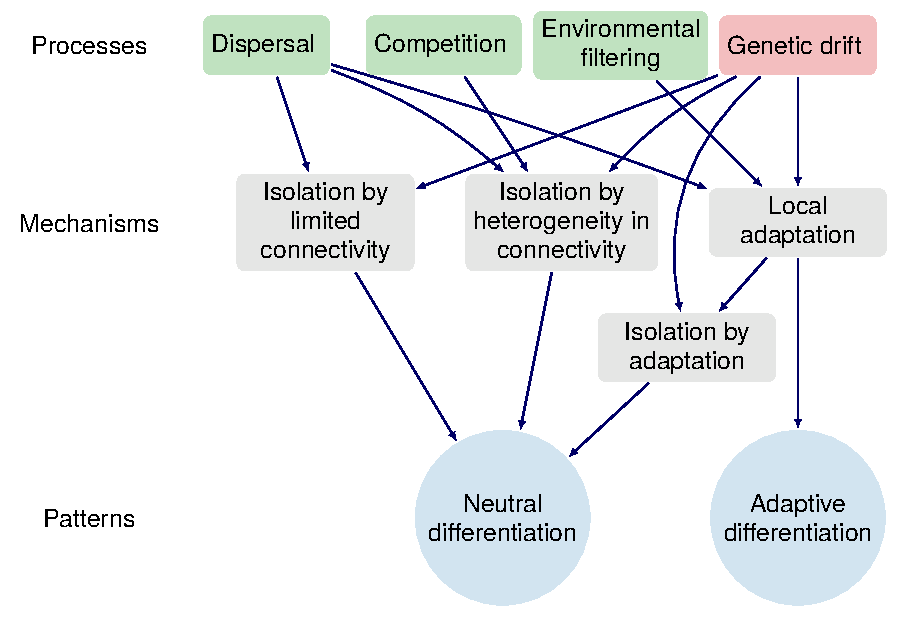
\includegraphics[width=\textwidth]{diff-in-graph.pdf}
    \caption{Summary of the causal pathways involved in neutral and adaptive differentation, disentangled in \chapi. Ecological processes are displayed in green boxes, evolutionary processes are displayed in red boxes.}
    \label{fig:summary_diff-in-graph}
\end{figure}


\subsubsection{Linking economic patterns to eco-evolutionary processes}

% Hypotheses concerning the processes that underly economic system dynamics are numerous, and have mainly been investigated through forward modelling. Starting from empirical observations, 
% 
\chapiii provides a novel understanding of the role of eco-evolutinoary processes in economic systems. %by assessing their effect on the dynamics of economic activities from data.
% 
% complements recent follows an inverse modelling approach to understand which processes are most likely shaping economic development. 
% 
Neoclassical economics and evolutionary economics seek to explain economic change with formal modelling, focusing on the relationships between economic variables such as output, employment and productivity \cite{Boschma2005a}.
% 
% Neoclassical economics sugggests that exogenous drivers, such as production costs, drive the diversification of economic systems \xxx. 
% 
In particular, evolutionary eonomics is concerned with explaining economic change by endogenous forces, such as interactions between firms and economic activities, and evolutionary processes acting upon them \cite{Hodgson2019,Metcalfe2006}.
% 
% Exogenous drivers, such as technological change \xxx, economic institutions \xxx, and production costs \cite{Boschma2005a} have been proposed, but 
% 
In opposition to this approach, complexity economics \cite{Hidalgo2021} seeks to predict variations in national income by using fine-grained data of economic activity outputs and dimensionality reduction techniques \cite{Mitchell}, without assumptions on the underlying processes \cite{Hidalgo}. 
% 
% One of the major contribution of complexity economics is to provide a metric that can predict economic development \cite{Taschella}, and the field is now concerned with understanding the factors underlying this factor.
%
While a current concern in evolutionary economics is to obtain an agreement between the mechanisms proposed and empirical observations \xxx, complexity economics seeks to understand the causal processes underlying the success of the dimensionality reduction technique \xxx.

By being agnostic to economic variables yet providing a causal link with the most probable processes underlying economic development, \chapiii bridges evolutionary economics and economic complexity.
% 
Our approach relies on the simple observation that the dynamics of economic activities contains signatures from the many complex processes that underpin them.
% 
These signatures consist in peculiar temporal variations and couplings that can be conveniently modelled by biologically inspired population dynamic models, which use are additionally justified by deep analogies between economic activities and biological populations. 
% 
Analogously to biological populations that are characterised by genes, economic activities are characterised by organizational routines \cite{NelsonWinter}, which experience evolutionary processes and define how they engage in ecological processes \cite{NelsonWinter}.
% 
% This connection is justified by evolutionary economics, which argues that similarly to genes, organizational routines are at the core of economic entities and experience ecological and evolutionary processes.
% 
As a result, and similarly to the size of biological populations, the capital growth of economic activites is determined by the ensemble of organizational routines that characterise them \cite{Boschma2005a}.
% 
Similarly to approaches used in ecology and evolution \cite{Skeels}, inverse modelling approaches can then be used to disentangle, from their signatures \cite{Skeels} left on the dynamics of economic activities, the role of the eco-evolutionary processes acting upon them.

%%
Specifically, \chapiii explores the effect of eco-evolutionary processes, proposed in the evolutionary economics and geography economics literature, on the dynamics of economic activities at the national scale.
% 
In particular, \chapiii seeks to test whether the dynamics of economic activities can be explained by different types of interdependencies, including positive \xxx and negative interactions \xxx, spatial transfers \xxx, and transformations \xxx.
% 
Using population dynamic models capturing the different interdependencies, \chapiii provides empirical evidence that economic activities engage in positive interactions, and benefit from spatial transfers of knowledge and routines.
% 
Positive interactions may arise from a variety of processes proposed in the evolutionary economic literature, such as supply chains \cite{Ozman2009,Saavedra2009a} and knowledge spillovers \cite{Menon2015}. 
% 
Its support implies that diversity promotes economic development \cite{Hidalgo2018}, as economic activities promote each other.
% 
The support for spatial transfers implies that, besides international patent laws \xxx, transfers of knowledge and organisational routines have a considerable on economic activities. Nevertheless, discrepancies in the strength of evidence obtained for spatial transfers across countries highlight that some countries are overall more akin to spatial transfers than others, which may be explained by differences in cognitive, organizational, social, institutional or geographic proximities across countries \xxx .
% 
I provide a summary of the mechanisms evidenced in economic systems in \cref{fig:summary_eco}. Overall, \chapiii bridges approaches in economics and biology to understand the mechanisms shaping the endogenous dynamics of economic systems.

% 
% The dynamics of economic activities contains signals from the many complex processes that underpin them, this approach enables to extract the effect of economic processes through their 

% for the diffusion of countries through the product space, explaining technological lock out.
% 
% by using data and dimensionality reduction technique to leverage these assumptions \cite{Taschella},

\subsection{Methodological advances in forward and inverse modelling}

\subsubsection{Advances in the modelling of realistic spatial and phenotypic structures}

\Cref{chapi,chapiv} provide new tools to better understand mechanisms resulting from ecological and evolutionary processes, and their interplay, in the context of realistic population structures and phenotypic distributions.
% 
% Population structure
Evolutionary dynamics have been traditionally studied in the context of homogeneous or spatially extended populations \cite{LiebermanHauert2005}.
% 
For instance, \cite{Slatkin1973,Slatkin1978,Kirkpatrick1997,Polechova2015,Polechova2018,AndradeRestrepo2019,Doebeli2003,Meszena1997,Yeaman2011,Debarre2013,Mirrahimi2020} consider regular spatial structures, missing the effect of the complexity of spatial structures on population differentiation.
% 
Nevertheless, biological habitats differ in their connectivity \xxx, and economic entities are structured through complex networks \xxx. The work of \cite{LiebermanHauert2005} and subsequent studies of "evolutionary dynamics on graphs" \xxx show that this complexity affects the interplay between selection and drift. However, evolutionary dynamics on graphs does not consider eco-evolutionary feedbacks \cite{Govaert2019a}.
% 
Thus far, models that include frequency dependence together with realistic, complex population structures were missing.

While a vast majory of the work on eco-evolutionary feedbacks has focused on the evolution of scalar phenotypes \cite{Doebeli2011}, in most organisms many phenotypic properties combine in complicated wasy to determin ecological interactions, and hence frequency-dependent selection \cite{Doebeli2014}
% 
\cite{Doebeli2011} shows that the consideration of multiple traits with complex interactions relaxes the unrealistic conditions of strong frequency dependence required to generate diversity in one dimensional phenotype spaces, calling for a better understanding of evolutionary dynamics in high dimensioanl spaces.
% 
\Cref{chapi} demonstrates that the co-evolution of traits proved to have genuine consequences on differentiation, pointing towards the inclusion of multiple traits to understand the dynamics of ecological interactions.
% 
Other works on eco-evolutionary dynamics, including cancer cell evolution \xxx and plankton dymamics \xxx, highlight the importance of considering multiple traits.
% 
The simulation of high dimensional models of trait leads to complications, since the numerical cost of traditional methods grows exponentially in the number of dimensions. 
% 
Novel numerical methods have been proposed to simulate high dimensional models, but they could not handle non-local terms, which capture non-local interactions between microscopic agents.

\cref{chapi} develops a generic modelling framework to capture the effect of eco-evolutionary processes on biological populations structured in complex landscapes, and \cref{chapiv} provides tools to efficiently simulate the resulting high-dimensional models.
% 
%% IBM
The IBM presented in \chapi involves the combination of graphs and highly dimensional phenotypic spaces, together with eco-evolutionary feedbacks, to model population structures. The modelling framework presented can readily be generalised, and the code associated to the numerical experiments in \chapi include a Julia library, \textbf{Evoid.jl}, that implements a more general version of the model. %(), 
% 
As such, the modelling framework presented in \chapi may be used to investigate other questions involving complex population structures and the co-evolution of characterisitcs.

% 
%% PDE
Reproducing the discrete and stochastic nature of ecological and evolutionary processes \cite{Champagnat2006}, simulations of the IBM may not provide a general understanding of system investigated \xxx, and cannot be scaled to simulate large systems involving millions of individuals \xxx. Nevertheless, the IBM proposed in \chapi is mathematically tractable under simplifying assumptions, and can be efficiently simulation with a deterministic PDE approximation.
% 
Tractability allows to obtain analytical insights on how structural properties affect macroscopic population under simplifying assumptions (\chapi).
% 
The PDE approximation, combined with the numerical methods presented in \chapiv, further allow efficient simulations. 
% 
I have implemented the numerial methods for simulating high dimensional models in the Julia library \textbf{HighDimPDE.jl} \cite{HighDimPDE}, a registered Julia package belonging to the SciML organisation \cite{XXX}.
%% 
The user interface respects standards from the SciML organisation, meaning that Julia users can easily adopt it.
%
The package aim at hosting any solver algorithms that break down the curse of dimensionality, and is currently receiving contributions to implement the DeepBSDE scheme \cite{Han2018}.

%% Conclusion
The combination of analytical insights and numerical simulations can help to elucidate the links between microscopic processes and macroscopic properties \cite{Levin}.
% 
\cref{chapi,chapiv} provide novel analytical and numerical tools to link the interplay between eco-evolutionary processes and complex spatio-evolutionary structures to the resulting mechanisms and patterns.


\subsubsection{Advances in inference methods for the investigation of eco-evoluationary processes}

\cref{chapii,chapiii} develop and test a novel inverse modelling method that allows to infer highly nonlinear dynamical processes from observation data. The method opens up new venues to further our understanding of the dynamics of biological and economic systems, and to provide predictions.
% 
The most developed inference methods in current use for inverse modelling are Bayesian inference methods with Markov Chain Monte Carlo \xxx and variational methods \xxx.
% 
% Bayesian inference methods with Markov Chain Monte Carlo \xxx and variational methods \xxx have been used since the past 20 years to calibrate dynamic ecosystem models \cite{Schartau2017}.
% 
Bayesian inference methods require a large number of forward model integrations \cite{Schneider2017}, and are highly affected by the number of model parameters \cite{Csillery2010}.
% 
Variational methods require the model sensitivity to its parameters \xxx and are prone to converge to local minima, especially with complex models \cite{XXX}.
% 
Those central issues likely explain the very poor number of studies that have used inverse modelling to further our knowledge on eco-evolutionary dynamics \xxx. 
% 

%
%% Our method
\chapii presents a novel inference framework that can handle with high computational efficiency dynamic eco-evolutionary models.
% 
The framework is based on a simple variational method, but relies on recent development in ML, including AD \cite{Rackauckas2020a} and state-of-the-art optimizers \cite{Kingma2014}, and implements a learning strategy based on a mini-batch method, in order to circumvent the drawbacks of variational methods and adapt to the specificities of eco-evolutionary models. 
% 
The use of AD simply eliminates the effort required to obtain the model sensitivity to its parameters, and the state-of-the-art optimizers, together with the mini-batch method, ensure the efficiency and reliably of the method in handling highly nonlinear models.
% 
By contrasting competing hypotheses embedded in alternative models, \cref{chapii,chapiv} provide concrete examples, both with synthetic and empirical data, that the ML framework can succesfully elucidate eco-evolutionary mechanistic pathways.
% 
This work is part of an ongoing effort to blend ML and traditional models to gain scientific understanding and extrapolability \cite{XXX}. Importantly, in contrast to physical systems such as ocean and atmospheric systems \xxx, invariant laws are yet to be formulated (if they exist). While ML is mostly used to improve model forecast skill in weather and climate modelling \xxx, the fields of Biology and Economic can gain scientific knowledge through model selection. 
% 
Nevertheless, the proposed method is also relevant for improving the forecast of predictive eco-evolutionary model \cite{Urban2016}, and integrates the practical constraints of datasets including short time series with partial, noisy, shallow and independent observations \cite{Dornelas2018}.

The ML framework is implemented in the multi-purpose Julia package \textbf{MiniBatchInference.jl} \cite{MiniBatchInference}, readily available to the scientific community. \textbf{MiniBatchInference.jl} is built around the celebrated differential equation solver \textbf{DifferentialEquations.jl} and the deep learning library \textbf{Flux.jl}. As such, the use of \textbf{MiniBatchInference.jl} requires very limited efforts to any user familiar with those libraries.

Overall, the method proposed in \cref{chapii} successfully blends ML methods with mechanistic ecosystem models to improve our gain scientific knowledge from observation data. Concret case examples in \cref{chapii, chapiii} show that it enables the testing of eco-evolutionary theories against data, advancing our understanding and the improvement of current mechanistic models, with the potential to provide better forecasts of ecosystems states \cite{Urban2016}.


\printbibliography[heading=subbibliography]
% \subsection{Blending ML and mechanistic models to learn from data}

% \subsection{Quantitative support for eco-evolutionary processes in economic systems}

% \subsection{Novel methods for the modelling of complex adaptive systems}


% \section{Limitations}

% \subsection{Limitation of PDE methods}
% \cite{Akesson2021} : PDE methods are probably not as adapted as trait based ODEs. Those simpler models can already address important questions regarding climate change.
% \cite{Tacchella2018}: In many cases, not only in economics, theoretical modelling and forecasting are not tightly related5
% . Most of the modelling efforts are
% in the direction of oversimplified representations that aim only at understanding the potential effects of a single variable, or of a lim- ited set of them, in a controlled setting

% \section{Conclusion}
% In light of the results, XXX.
% % 
% We expect XXX.

% %%
% Consequently, this thesis contributed to a better understanding of XXX.
% % 
% While recent studies have underlined the need to account for XXX, we XX.

% \section{Perspectives}

% \subsection{Toward a continuum between ML and mechanistic models}

% \subsection{Evolutionary biology to undertsand the economic patterns}


% \subsubsection*{An urgent need for better understanding and model eco-evolutionary dynamics}
% The effect of direct anthropogenic pressure, together with climate change, is rapidly affecting ecosystems \cite{Ellis2011,Midgley2019}. Ecosystems are approaching state shifts \cite{Barnosky2011,Barnosky2012,Midgley2019}, which in turn will greatly affect human societies \cite{Mooney2009}.
% %
% %% Constatation of system state shift
% % Current extinction rates are higher than would be expected from the fossil record \cite{Barnosky2011}. %Based on habitat models, \cite{Midgley2019} predicts, on the basis of mid-range climate-warming scenarios for 2050, that 15\% to 37\% of species would be committed to extinction. 
% % 
% %%
% While there is a general agreement that anthropogenic pressure and climate change will have a negative effect on the biosphere \cite{fischlin2007ecosystems}, their precise effect on ecosytem dynamics is unclear \cite{Norberg2012}. In particular, the answer to how species will adapt to increasing temperatures is uncertain due to our lack of understanding of eco-evolutionary feedbacks \cite{Norberg2012}. 
% % 
% %For instance, with global warming, species are likey to shift towards higher elevations and higher latitudes \cite{Chen2011}. Because the speed of range shifts differ between different ecological groups, climate change is expected to modify the current organization of trophic interactions \cite{Descombes2020}, affecting ecosystem functioning.
% %
% %% 
% Current projections of ecosystem states, such as \cite{Midgley2019},
% are based on habitat models, where species habitats are deducted from species occurence data, and are reprojected it given environmental predictors.
% % 
% Such approaches miss the processes of ecological interactions, evolutionary change and species dispersal \cite{Pearson2003}, that are expected to play a critical role in the evolution of the biosphere in the coming decades \cite{Norberg2012}.
% % 
% In order to mitigate the consequences of human development, it is of utmost urgency to better understand eco-evolutionary feedbacks \cite{Norberg2012}, and develop mechanistic models embedding this knowledge \cite{Urban2016}. This will in turn provide more reliable forecasts of ecosystem states \cite{Clark2001}, to help designing adequate management of ecosystem services \cite{Urban2016}.

% % \subsubsection*{Endogenous forces in economic systems}
% % Traditional approaches to economics assume the rationality of economic agents \xxx. Economic dynamics
% % % 
% % In contrast, evolutionary economics 